\chapter{Đánh giá kết quả}

Một trong những nhiệm vụ quan trọng của việc huấn luyện là tiến hành đánh giá kết quả thu được. Việc đánh giá kết quả nhằm mục đích phân tích, đánh giá hiệu quả của các mô hình. Nhóm sẽ tiến hành đánh giá mô hình FCRN, đây là mô hình sinh depth map mà nhóm sử dụng để ước lượng khoảng cách. Bên cạnh đó, nhóm cũng sẽ tiến hành đánh giá kết quả của việc ước lượng khoảng cách vật thể dựa trên 2 cách tiếp cận mà nhóm đã đề xuất. Dựa vào các kết quả thu được, nhóm sẽ đưa ra các nhận xét, đề cập các nhược điểm mô hình gặp phải và đưa ra phương pháp điều chỉnh trong quá trình sinh ra depth map cũng như ước lượng khoảng cách vật thể. 

\section{Các chuẩn đo được dùng để đánh giá mô hình}

\subsection{Các chuẩn đo để đánh giá mô hình sinh depth map}

Trong việc đánh giá kết quả của mô hình FCRN nói riêng, hay các cấu trúc khác của mô hình sinh depth map, thì theo khảo sát của nhóm, các độ đo thường được sử dụng: root mean squared error(RMSE), mean absolute relative error(REL)  Thresholded accuracy\\ 


Dưới đây là những độ đo đánh giá về độ lỗi của mô hình, tại đó $y_i$ là giá trị thực tế ta có, còn $y_i^{*}$ là giá trị dự đoán từ mô hình, và $\left | T \right |$ là tổng số điểm ảnh trên toàn bộ những bức ảnh được đánh giá.
\begin{itemize}
\item RMSE: $\sqrt[]{\frac{1}{\left | T \right |} \sum _{y\in T}\left \|y_{i}-y_{i}^{*}  \right \|^{2}}$\\
Độ đo này còn có tên khác standard deviation of residuals, nó dùng để đánh giá độ sai biệt trung bình giữa giá trị dự đoán từ mô hình so với giá trị thực tế. Nếu giá trị này càng nhỏ thì độ chênh lệch trung bình giữa giá trị dự đoán với giá trị thực tế càng nhỏ, điều đó cho thấy mô hình dự đoán càng tốt.
%\item Root mean squared error log (rmslog): $\sqrt[]{\frac{1}{\left | T \right |} \sum _{y\in T}\left \|\log y_{i}- \log y_{i}^{*}  \right \|^{2}}$

\item Mean absolute relative error (rel): $\frac{1}{\left | T \right |} \sum _{y\in T} \left | y_i - y_i^{*} \right |/y_i$\\
Mặc dù đã có độ đo rms nhưng độ đo này nói lên giá trị trung bình của tỉ lệ độ chênh lệch giữa giá trị dự đoán $y^{*}$ và giá trị thực tế y so với giá trị thực tế y có nghĩa rằng ngoài việc biết được sự chênh lệch trung bình giữa giá trị dự đoán với giá trị thực tế  từ rms, ta còn muốn biết trung bình thì độ chênh lệch này so với giá trị thực tế là bao nhiêu lần.

\item Mean $\log_{10}$ error (log10): $\frac{1}{\left | T \right |} \sum _{y\in T}\left | \log_{10}y_i- \log_{10}y_i^{*}  \right |$\\
 Bời vì $\left | \log_{10}y_i- \log_{10}y_i^{*}  \right | = \left | \log_{10}\frac{y_i}{y_i^{*}}  \right |$ do đó độ đo này cho biết trung bình thì giá trị tỉ lệ của độ sâu dự đoán và độ sâu thực tế ở dạng $log_{10}$.
\end{itemize}

Để đánh giá độ chính xác của mô hình sinh depth map ta dùng độ chính xác theo ngưỡng (accuracy with threshold):\\
\begin{itemize}
\item Relative error: $\max \left \{ \frac{y_i^{*}}{y_i}, \frac{y_i}{y_i^{*}} \right \}$\\
Độ lỗi này được dùng để đánh giá xem giá trị độ sâu mà mô hình dự đoán có chính xác hay không tùy thuộc vào ngưỡng mà ta cho trước. Cụ thể, với mỗi giá trị độ sâu được dự đoán ta sẽ có được độ lỗi theo relative error, nếu giá trị này nhỏ hơn theo giá trị của ngưỡng cho trước $\delta$ thì ta xem mô hình đã dự đoán chính xác độ sâu tại điểm ảnh đó.

%Đ tỉ lệ của $y^{i} $, $\max(\frac{y_i}{y_i^{*}},\frac{y_i^{*}}{y_i}) = \delta^{k} < threshold$ với k = 1, 2, 3\\
\item $\delta_i$: là phần trăm của những điểm ảnh mà mô hình đã dự đoán chính xác độ sâu so với tất cả những điểm mà mô hình đã đưa ra dự đoán, cụ thể ta có công thức sau,
 \begin{center}
 $\delta_i = \frac{\mathbf{card}\left ( \left \{ y_i^{*}:  \max \left \{ \frac{y_i^{*}}{y_i}, \frac{y_i}{y_i^{*}} \right \}  < 1.25^{i} \right \} \right )}{\mathbf{card}\left ( \left \{ y_i \right \} \right )}$
 \end{center}
 Ở đây $\mathbf{card}$ là số lượng phần tử của tập hợp, và ngưỡng của  độ chính xác $\delta_i$ là $1.25^{i}$. Các công trình mà nhóm khảo sát thường chọn 3 độ chính xác để đánh giá mô hình với i tương ứng là 1, 2 và 3
\end{itemize}
\subsection{Các chuẩn đo để đánh giá kết quả của việc ước lượng khoảng cách}
Khác với việc đánh giá kết quả dựa trên ground truth, thì việc ước lượng khoảng cách của nhóm sẽ dựa trên việc so sánh 2 cách tiếp cận khác nhau mà nhóm đã đề xuất. Những đánh giá sơ bộ của nhóm dựa trên các giá trị: min, max, mean, standard deviation.

\section{Đánh giá kết quả}
\subsection{Đánh giá kiến trúc của mô hình ước lượng độ sâu}

Để đánh giá kiến trúc của mô hình ước lượng độ sâu, nhóm sẽ tiến hành khảo sát sự ảnh hưởng của những hàm mất mát khác nhau, những kiến trúc decoder khác nhau dựa trên độ chính xác của kết quả dự đoán ảnh độ sâu trên tập xác thực

\begin{enumerate}
\item Hàm mất mát: Để đánh giá hiệu quả của các hàm mất mát, nhóm đã sử dụng cùng một kiến trúc, ở đây với decoder là lớp deconvolution kernel size $2x2$. Các hàm mất mát được nhóm đánh giá bao gồm: hàm $L_1$, $L_2$, berHu.
\begin{table}[H]
\centering
\begin{tabular}{ |p{1.5cm}|p{1.5cm}|p{1.5cm}|p{1cm}|p{1cm}|p{1cm}|p{1cm}|p{1cm}|p{1cm}|}
% \hline
% \multicolumn{3}{|c|}{Country List} \\|p{1cm}
\hline
Loss & Encoder &  Decoder & RMSE &  REL & log10 & $\delta_1$ & $\delta_2$ & $\delta_3$ \\
\hline
$L_1$ & Conv & Deconv2 & 0.652 & 0.196 & nan & 69.6 & 92.4 & 98.1 \\
\hline
$L_2$ & Conv &  Deconv2  & 0.717 & 0.229 & 0.093 & 62.2 & 89.6 & 97.3\\
\hline
berHu & Conv & Deconv2 & 0.633 & 0.195 & 0.079 & 70.8 & 92.7 & 98.1 \\
\hline
\end{tabular}
\caption{Sự ảnh hưởng từ các hàm mất mát đến kết quả dự đoán}
\label{tab:compare_loss}
\end{table}
Từ kết quả trên ta thấy hàm mất mát berHu cho kết quả tốt hơn 2 hàm còn lại, nên nhóm sẽ chọn hàm berHu là hàm mất mát cho quá trình huấn luyện từ đây trở về sau. Chúng ta cần chú ý giá trị nan ở độ lỗi log10 của $L_1$ gây ra là do mô hình đã dự đoán một giá trị khoảng cách âm tại một điểm ảnh nào đó nên kết quả độ lỗi log10 toàn cục là nan.
\item Kiến trúc decoder: Dựa vào kết quả của bảng \ref{tab:compare_loss}, nhóm đã chọn được hàm mất mát. Tiếp theo, từ những decoder đã được đề xuất, bao gồm: deconvolution 2, deconvolution 3, upconvolution và upprojection, nhóm sẽ tiến hành đánh giá và chọn ra decoder cho kết quả tốt nhất. Từ kết quả ở bảng \ref{tab:compare_decoder} ta thấy Deconv3 có kích thước kernel là $3\times3$ cho kết quả khá tương tự Deconv2 có kích thước kernel $2\times2$, đồng thời Upproj có vẻ tốt hơn một ít so với Upconv và bọn chúng tốt hơn hẳn Deconv3 và Deconv2, nên nhóm đi đến quyết định chọn kiến trúc Upproj làm kiến trúc cho bộ decoder cho những thí nghiệm trở về sau.

\begin{table}[H]
\centering
\begin{tabular}{ |p{1.5cm}|p{1.5cm}|p{1.5cm}|p{1cm}|p{1cm}|p{1cm}|p{1cm}|p{1cm}|}
% \hline
% \multicolumn{3}{|c|}{Country List} \\
\hline
Encoder &  Decoder & RMSE &  REL & log10  &$\delta_1$ & $\delta_2$ & $\delta_3$ \\
\hline
Conv & Deconv2 & 0.633 & 0.195 & 0.078 & 70.8 & 92.7 & 98.1 \\
\hline
 Conv &  Deconv3  & 0.632 & 0.196 & 0.079 &  70.2 & 92.7 & 98.1\\
\hline
 Conv & Upconv & 0.607 & 0.185 & 0.075 & 72.6 & 93.6 & 98.3 \\
\hline
Conv & Upproj & 0.606 & 0.182 & 0.075 & 72.6 & 93.3 & 98.4 \\
\hline
\end{tabular}
\caption{Sự ảnh hưởng của các decoder tới kết quả dự đoán}
\label{tab:compare_decoder}
\end{table}
% phải gõ thêm để hoàn thiện 
\end{enumerate} 

\subsection{Đánh giá kết quả ước lượng độ sâu}
Từ kết quả của việc đánh giá các hàm mất mát cũng như kiến trúc decoder của mô hình, nhóm sẽ tiến hành khảo sát sự ảnh hưởng của số lượng mẫu độ sâu lên chất lượng của kết quả dự đoán ảnh độ sâu. Nhóm sẽ tiến hành thử nghiệm với số mẫu tăng dần từ 0, 100, 200, 500, 700, 800, 1000, 2000, 3000, 5000. 
Sau khi chọn được hàm mất mát là berHu và kiến trúc decoder là Upprojection phục vụ cho quá trình huấn luyện. Nhóm sẽ tiến hành khảo sát sự ảnh hưởng của số lượng mẫu độ sâu lên chất lượng của kết quả dự đoán của mô hình, 


\begin{enumerate}
\item Deconvolution 2: mô hình sử dụng decoder là  deconvolution 2, hàm loss l1. Nhóm sẽ tiến hành thử nghiệm với các giá trị sampling depth khác nhau. 
% \begin{center}
\begin{table}[H]
\centering
\begin{tabular}{ |p{3cm}|p{1.5cm}|p{1.5cm}|p{1cm}|p{1cm}|p{1cm}|p{1cm}|   }
% \hline
% \multicolumn{3}{|c|}{Country List} \\
\hline
Mô hình & RMSE &  REL & log10 & $\delta_1$ & $\delta_2$ & $\delta_3$ \\
\hline
RGB & 0.621 & 0.186 & 0.076 & 72.7 & 93.0 & 98.2 \\
\hline
RGB+100 mẫu & 0.362 &  0.089  & 0.038 & 92.1 & 98.4 & 99.6\\
\hline
RGB+200 mẫu & 0.305 & 0.076 & 0.032 & 94.4 & 99.0 & 99.8 \\
\hline
RGB+500 mẫu & 0.290 & 0.071 & 0.030 & 95.0 & 99.2 & 99.8\\
\hline
RGB+700 mẫu & 0.280 & 0.068 & 0.029 & 95.4 & 99.3 & 99.8\\
\hline
RGB+800 mẫu & 0.304 & 0.074 & 0.032 & 94.9 & 99.2 & 99.8\\
\hline
RGB+1000 mẫu & 0.279 & 0.068 & 0.029 & 95.4 & 99.2 & 99.8\\
\hline
RGB+2000 mẫu & 0.284 & 0.069 & 0.029 & 95.5 & 99.3 & 99.8\\
\hline 
RGB+3000 mẫu & 0.282 & 0.068 & 0.029 & 95.7 & 99.4 & 99.9\\
\hline
RGB+5000 mẫu & 0.268 & 0.065 & 0.028 & 95.8 & 99.3 & 99.9\\
\hline
RGB+10000 mẫu & 0.261 & 0.064 & 0.027 & 96.0 & 99.4 & 99.9\\
\hline
\end{tabular}
\caption{So sánh kết quả trong kết quả mô hình sử dụng decoder deconvolution}
\label{tab:deconv2}
\end{table}
% \end{center}
% \includegraphics[width=\paperwidth,height=\textheight]{image/deconv2_s200}
 \begin{center}
   \begin{figure}[H]
   \begin{center}
   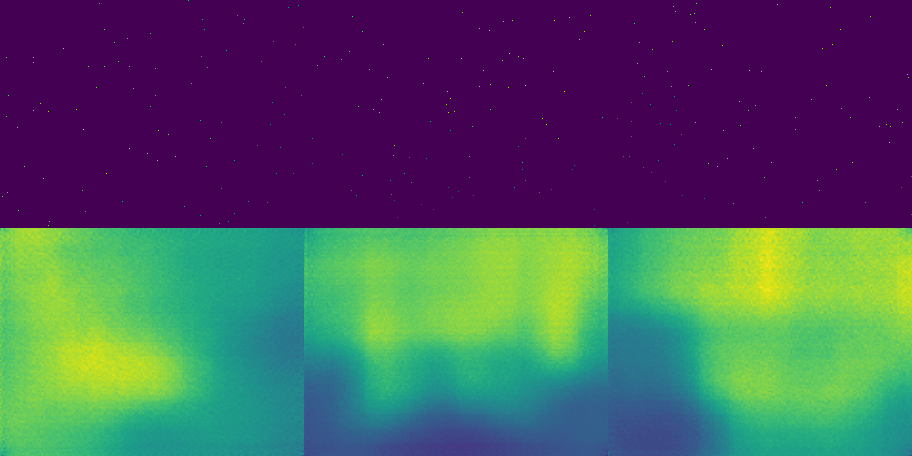
\includegraphics[scale=0.5]{image/100sample}
% \includegraphics[width=\paperwidth,height=\textheight]{image/deconv2_s200}
   \end{center}
   \caption[Kết quả so sánh khi dự đoán ảnh độ sâu với 200 điểm sampling dùng deconvolution 2]{Kết quả so sánh khi dự đoán ảnh độ sâu với 200 điểm sampling dùng deconvolution 2. Ảnh trong cột đầu tiên mô tả ảnh gốc RGB, ảnh thưa được thể hiện ở cột thứ 2. Trong cột thứ 3 và thứ 4 lần lượt là ground truth ảnh độ sâu và ảnh độ sâu được dự đoán khi sử dụng mô hình}
   \label{fig:deconv2_s200}
   \end{figure}
 \end{center}
 
%  \begin{center}
%    \begin{figure}[H]
%    \begin{center}
%    \includegraphics[scale=0.5]{image/comparison_169}
%    \end{center}
%    \caption{Kết quả so sánh khi dự đoán ảnh độ sâu với 100 điểm sampling dùng deconvolution 2.}
%    \label{fig:deconv2_100s}
%    \end{figure}
%  \end{center}
 
 \begin{center}
   \begin{figure}[H]
   \begin{center}
   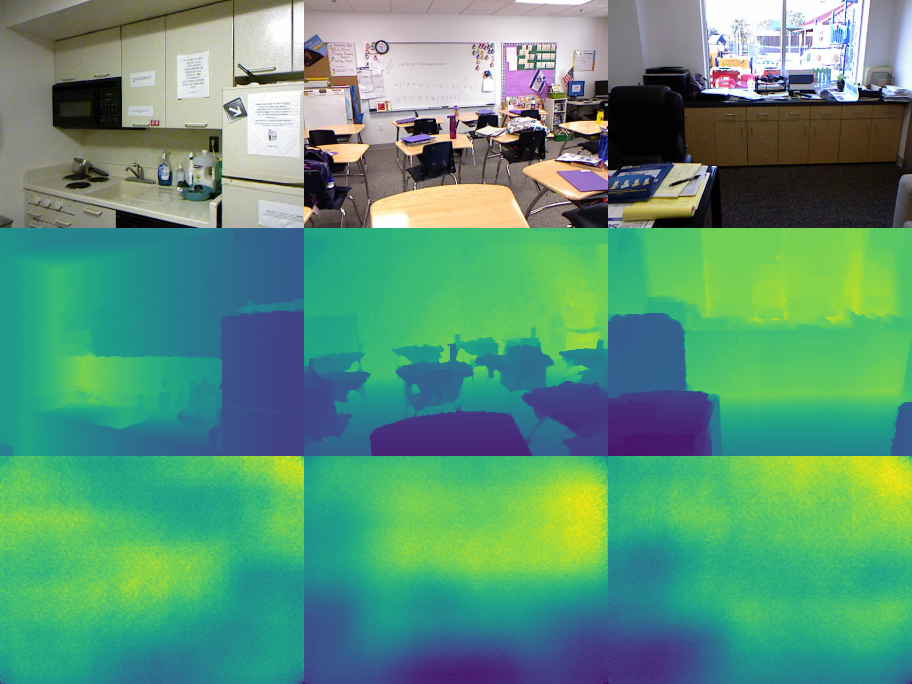
\includegraphics[scale=0.5]{image/0sample}
   \end{center}
   \caption[abcdef]{Kết quả so sánh khi dự đoán ảnh độ sâu với chỉ từ ảnh RGB dùng deconvolution 2}
   \label{fig:deconv2_0s}
   \end{figure}
 \end{center}

\item Deconvolution 3: mô hình sử dụng decoder là  deconvolution 3, hàm loss l1. Nhóm sẽ tiến hành thử nghiệm với các giá trị sampling depth khác nhau. 
% \begin{center}
\begin{table}[H]
\centering
\begin{tabular}{ |p{4cm}|p{2.5cm}|p{2cm}|p{1cm}|p{1cm}|p{1cm}|   }
% \hline
% \multicolumn{3}{|c|}{Country List} \\
\hline
Mô hình & RMSE &  REL & $\delta_1$ & $\delta_2$ & $\delta_3$ \\
\hline
Deconv3+0 sampling & 0.764 & 0.188 & 0.696 & 0.9492 & 0.9879 \\
\hline
Deconv3+100sampling & 0.483 &  0.103  & 0.895 & 09.9767 & 0.9947\\
\hline
Deconv3+200sampling & 0.447 & 0.093 & 0.918 & 0.9733 & 0.9937 \\
\hline
\end{tabular}
\caption{So sánh kết quả trong kết quả mô hình sử dụng decoder deconvolution 3}
\label{tab:deconv3}
\end{table}
 
 
 \item Upconvolution: mô hình sử dụng decoder là  upconvolution 3, hàm loss l1. Nhóm sẽ tiến hành thử nghiệm với các giá trị sampling depth khác nhau. 
% \begin{center}
\begin{table}[H]
\centering
\begin{tabular}{ |p{4cm}|p{2.5cm}|p{2cm}|p{1cm}|p{1cm}|p{1cm}|   }
% \hline
% \multicolumn{3}{|c|}{Country List} \\
\hline
Mô hình & RMSE &  REL & $\delta_1$ & $\delta_2$ & $\delta_3$ \\
\hline
Upconv+0 sampling & 0.808 & 0.198 & 0.604 & 0.9492 & 0.9879 \\
\hline
Upconv+100sampling & 0.461 &  0.099  & 0.902 & 09.9767 & 0.9947\\
\hline
Upconv+200sampling & 0.431 & 0.096 & 0.912 & 0.9733 & 0.9937 \\
\hline
\end{tabular}
\caption{So sánh kết quả trong kết quả mô hình sử dụng decoder upconvolution}
\label{tab:upconv}
\end{table}
 

\item Upprojection: mô hình sử dụng decoder là  upprojection, hàm loss l1. Nhóm sẽ tiến hành thử nghiệm với các giá trị sampling depth khác nhau. 
% \begin{center}
\begin{table}[H]
\centering
\begin{tabular}{ |p{4cm}|p{2.5cm}|p{2cm}|p{1cm}|p{1cm}|p{1cm}|   }
% \hline
% \multicolumn{3}{|c|}{Country List} \\
\hline
Mô hình & RMSE &  REL & $\delta_1$ & $\delta_2$ & $\delta_3$ \\
\hline
Upproj+0 sampling & 0.948 & 0.237 & 0.575 & 0.9492 & 0.9879 \\
\hline
Upproj+100sampling & 0.484 &  0.111  & 0.883 & 09.9767 & 0.9947\\
\hline
Upproj+200sampling & 0.496& 0.113 & 0.883 & 0.9733 & 0.9937 \\
\hline
\end{tabular}
\caption{So sánh kết quả trong kết quả mô hình sử dụng decoder upprojection}
\label{tab:upproj}
\end{table}
 
\end{enumerate}

\subsection{Đánh giá giá trị khoảng cách}
Các cách ước lượng khoảng cách vật thể mà nhóm đã đề xuất chủ yếu dựa trên kinh nghiệm, đồng thời, khoảng cách của những đối tượng trong ảnh đến camera cũng không được đánh nhãn. Do đó, nhóm chỉ có thể tiến hành đánh giá, so sánh các giá trị khoảng cách giữa các phương pháp với nhau. Các cách ước lượng khoảng cách mà nhóm đã hiện thực: lấy mẫu những điểm xung quanh tâm bao đóng của vật thể theo phân bố Gaussian ($all\_rdp$), lấy tất cả những điểm là kết quả của phân đoạn bằng Mask RCNN ($all\_mask$), lấy tất cả những điểm phân bố ngẫu nhiên thuộc kết quả phân đoạn Mask RCNN ($rdp\_mask$). \\ 

Từ tập dữ liệu NYUV2, nhóm chỉ chọn các hình ảnh có chứa những đối tượng: chai nước, giường ngủ và toi-let. Khi áp dụng mô hình FCRN và Mask RCNN trên tập ảnh này, nhóm thu được khoảng cách của 971 đối tượng bao gồm cả 3 loại trên. \\

% \begin{enumerate}[noitemsep]
\hspace{.2cm}\textbf{1. Tiến hành đánh giá sự chênh lệch khoảng cách của các phương pháp}: dựa trên khoảng cách đạt được từ ảnh độ sâu thực tế và ảnh độ sâu được dự đoán qua mô hình FCRN. Việc đánh giá sẽ tiến hành trên các đoạn khoảng cách khác nhau, bao gồm: 0 đến 1m, 1m đến 2m, 2m đến 3m, 3m đến 4m, 4m đến 5m, và lớn hơn 5m. Ví dụ: có khoảng 35 đối tượng nằm trong khoảng cách từ 0->1m(lấy dựa trên khoảng cách lấy được từ ảnh độ sâu thực tế). Từ đó, tính ra độ chênh lệch của những đối tượng đó giữa khoảng cách từ ảnh độ sâu thực tế và ảnh độ sâu được dự đoán và lấy giá trị trung bình của những giá trị chênh lệch này. 
\begin{table}[H]
\centering
\begin{tabular}{ |p{3cm}|p{1.5cm}|p{1.5cm}|p{1.5cm}|p{1.5cm}|p{1.5cm}|p{1.5cm}|}
% \hline
% \multicolumn{3}{|c|}{Country List} \\
\hline
PP đánh giá & 0-1m &  1-2m & 2-3m & 3-4m & 4-5m & >5m \\
\hline
$All\_rdp$ & 0.126 & 0.102 & 0.103 & 0.180 & 0.312 & 0.397 \\
\hline
$All\_mask$ & 0.121 &  0.106  & 0.111 & 0.168 & 0.305 & 0.374\\
\hline
$Rdp\_mask$ & 0.132& 0.111 & 0.116 & 0.188 & 0.314  & 0.422\\
\hline
\end{tabular}
\caption{So sánh sự chêch lệch giữa khoảng cách từ ảnh độ sâu thực tế và ảnh được dự đoán theo từng phương pháp}

\label{tab:compare_gtpred}
\end{table}

Theo kết quả từ bảng \ref{tab:compare_gtpred}, có thể thấy sự chênh lệch khoảng cách vật thể trong ảnh độ sâu thực tế và ảnh dự đoán là dựa vào độ chính xác của việc dự đoán ảnh độ sâu. Với những vật nằm ở khoảng cách càng xa camera, sự chính xác trong việc dự đoán ảnh độ sâu càng giảm, dẫn tới sự chênh lệch trong việc dự đoán khoảng cách vật thể từ ảnh độ sâu thực tế và ảnh độ sâu dự đoán là càng lớn. Bên cạnh đó, từ kết quả của bảng trên, nhóm cũng thấy rằng khi vật thể nằm trong khoảng từ 1-3 mét, sự chênh lệch của việc dự đoán khoảng cách từ ảnh độ sâu thực tế và ảnh độ sâu dự đoán là nhỏ nhất. Mặt khác, nếu vật ở quá gần camera, chẳng hạn như đoạn 0-1m, thì sự chênh lệch của khoảng cách lại lớn hơn so với đoạn từ 1-3m . Hình \ref{fig:deviation} thể hiện trực quan sự thay đổi của độ chênh lệch khoảng cách giữa ảnh độ sâu thực tế và ảnh độ sâu dự đoán của các phương pháp đo khoảng cách mà nhóm đề xuất.  

\begin{center}
   \begin{figure}[H]
   \begin{center}
   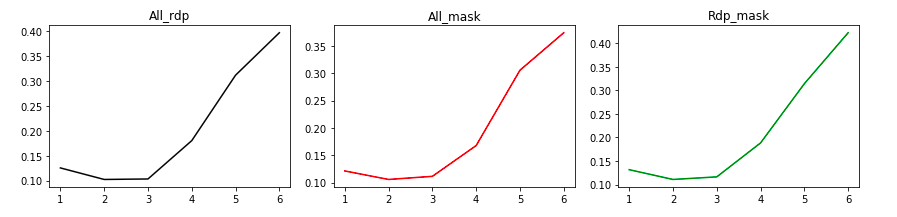
\includegraphics[scale=0.55]{image/deviation}
   \end{center}
   \caption{Sự chênh lệch khoảng cách giữa ảnh độ sâu thực tế và ảnh dự đoán}
   \label{fig:deviation}
   \end{figure}
 \end{center}
 
 Các giá trị trong bảng \ref{tab:compare_gtpred} là giá trị trung bình của sự chênh lệch khoảng cách thuộc đoạn, do đó giá trị trên là khá lớn vì trong mỗi đoạn đều sẽ chứa những nhiễu gây ảnh hưởng đến giá trị mà ta thu được. Hình \ref{fig:distribution} thể hiện rõ hơn sự phân bố của những giá trị chênh lệch này. Nhóm đã tiến hành đếm số lượng sự chênh lệch khoảng cách giữa ảnh độ sâu thực tế và ảnh dự đoán.  Ví dụ, trong phương pháp $all\_rdp$ có khoảng 221 độ chênh lệch khoảng cách nằm trong đoạn từ 0m đến 0.03m, khoảng 183 độ chênh lệch khoảng cách cách nằm trong đoạn từ 0.03m đến 0.06m... \\
 
 Từ đây, nhóm thấy rằng sự chênh lệch các giá trị khoảng cách là không quá lớn, đa số các độ chênh lệch tập trung vào khoảng sai số từ 0m đến 0.2m.Tuy nhiên, vẫn có một vài trường hợp cho ta thấy sự chênh lệch khá lớn. Một trong những lý do chính có thể dẫn đến sự chênh lệch này có thể là do kết quả dự đoán ảnh độ sâu có sự sai khác lớn đối với ảnh thực tế.
 \begin{center}
   \begin{figure}[H]
   \begin{center}
   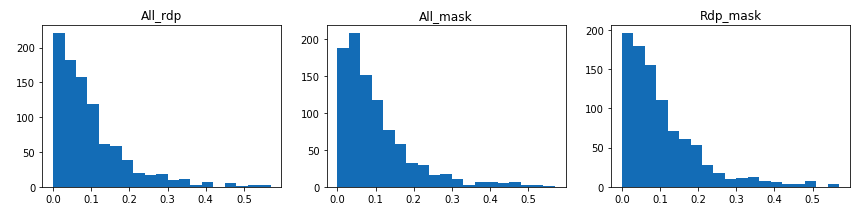
\includegraphics[scale=0.55]{image/distribution}
   \end{center}
   \caption{Sự chênh lệch khoảng cách giữa ảnh độ sâu thực tế và ảnh dự đoán}
   \label{fig:distribution}
   \end{figure}
 \end{center} 
 \hspace{.2cm}\textbf{2. Tiến hành đánh giá sự ảnh hưởng của hình dạng vật thể với kết quả dự đoán ảnh độ sâu}: những vật thể mà nhóm chọn để đánh giá bao gồm: chai nước, giường ngủ và toi-let. Mỗi vật thể trên đều có hình dáng rất khác nhau. Số lượng vật thể mà Mask RCNN phát hiện trên được vào khoảng 970 vật thể, trong đó có khoảng 635 chai nước, 260 giường ngủ và khoảng 75 toi-let. \\
 
Nhóm đã chọn kết quả phân đoạn từ Mask RCNN làm kết quả bề mặt của vật thể  và tiến hành phân tích bằng cách chọn giá trị độ sâu lớn nhất và nhỏ nhất của những bề mặt vật thể này trên ảnh độ sâu thực tế. Sau đó tiến hành so sánh giữa độ chênh lệch của giá trị lớn nhất, giá trị nhỏ nhất này trên từng loại vật thể.
\begin{center}
   \begin{figure}[H]
   \begin{center}
   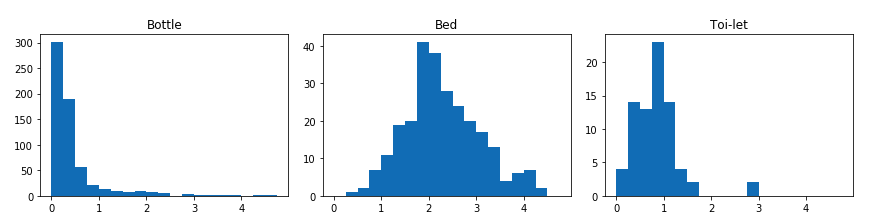
\includegraphics[scale=0.55]{image/gtminmax}
   \end{center}
   \caption{Sự chênh lệch giá trị lớn nhất, nhỏ nhất của vật thể trên ảnh độ sâu thực tế}
   \label{fig:gtminmax}
   \end{figure}
 \end{center} 
 
 Từ hình \ref{fig:gtminmax}, với vật thể là chai nước thì có khoảng hơn 500 giá trị chênh lệch giữa giá trị lớn nhất và nhỏ nhất là nhỏ hơn 0.5m. Mặt khác, với những vật thể có kích thước lớn cả về chiều rộng và chiều dài, thì độ chênh lệch sẽ được thể hiện càng lớn. Ở kết quả thống kê của nhóm với đối tượng là cái giường ngủ, thì có khoảng 170 giá trị chênh lệch nằm trong khoảng từ 1.75m đến 2.5m. Với đối tượng cuối cùng là toi-let với hình dạng phức tạp hơn, thì đa số sự chênh lệch này tập trung vào khoảng từ 0.5m đến 1m. Từ những kết quả nhận được trong hình \ref{fig:gtminmax}, ta có thể thấy rằng những tính chất về hình dạng của vật thể  được thể hiện khá rõ trên ảnh độ sâu. 

 
 